\documentclass[border=10pt]{standalone}
\usepackage{pgfplots}
\pgfplotsset{compat=1.18}
\begin{document}
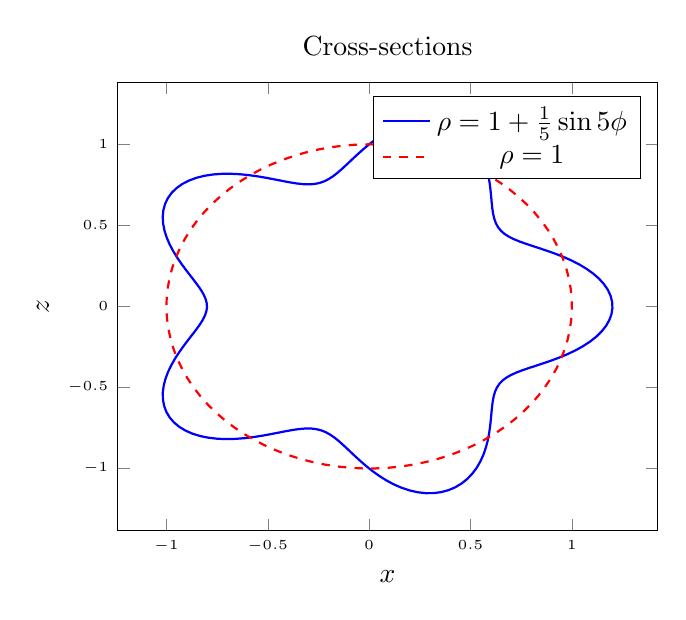
\begin{tikzpicture}
\begin{axis}[xlabel={$x$}, ylabel={$z$}, title={Cross-sections}, legend pos=north east, tick label style={font=\tiny}]
\addplot[blue, thick, domain=0:360, samples=200]
({(1 + 0.2*sin(5*x))*sin(x)}, {(1 + 0.2*sin(5*x))*cos(x)});
\addlegendentry{$\rho = 1+\frac{1}{5}\sin 5\phi$}
\addplot[red, dashed, thick, domain=0:360, samples=100]
({sin(x)}, {cos(x)});
\addlegendentry{$\rho = 1$}
\end{axis}
\end{tikzpicture}
\end{document}
